
\chapter{\textit{Doctor Strangeflow}, or how I learned to relax and love Reynolds numbers}


Of all the non-analytical (non-chemistry) process measurements students encounter in their Instrumentation training, flow measurement is one of the most mysterious.  Where else would we have to \textit{take the square root} of a transmitter signal just to measure a process variable in the simplest case?  Since flow measurement is so vital to many industries, it cannot go untouched in an Instrumentation curriculum.  Students must learn how to measure flow, and how to do it accurately.  The fact that it is a fundamentally complex thing, however, often leads to oversimplification in the classroom.  Such was definitely the case in my own education, and it lead to a number of misunderstandings that were corrected after a lapse of 15 years, in a sudden ``Aha!'' moment that I now wish to share with you.

The orifice plate is to flow measurement what a thermocouple is to temperature measurement: an inexpensive yet effective primary sensing element.  The concept is disarmingly simple.  Place a restriction in a pipe, then measure the resulting pressure drop ($\Delta P$) across that restriction to infer flow rate.  

\filbreak

You may have already seen a diagram such as the following, illustrating how an orifice plate works:

$$\includegraphics{flow01.eps}$$ \index{Vena contracta}

Now, the really weird thing about measuring flow this way is that the resulting $\Delta P$ signal does not linearly correspond to flow rate.  Double the flow rate, and the $\Delta P$ quadruples.  Triple the flow rate and the $\Delta P$ increases by a factor of nine.  To express this relationship mathematically:

$$Q^2 \propto \Delta P$$

In other words, differential pressure across an orifice plate ($\Delta P$) is proportional to the \textit{square} of the flow rate ($Q^2$).  To be more precise, we may include a coefficient ($k$) with a precise value that turns the proportionality into an equality:

$$Q^2 = k(\Delta P)$$

\filbreak

Expressed in graphical form, the function looks like one-half of a parabola:

$$\includegraphics{flow02.eps}$$

To obtain a linear flow measurement signal from the differential pressure instrument's output signal, we must ``square root'' that signal, either with a computer inside the transmitter, with a computer inside the receiving instrument, or a separate computing instrument (a ``square root extractor'').  We may see mathematically how this yields a value for flow rate ($Q$), following from our original equation: \index{Square root characterizer}

$$Q^2 = k(\Delta P)$$

$$\sqrt{Q^2} = \sqrt{k(\Delta P)}$$

$$Q = \sqrt{k(\Delta P)}$$

\vskip 5pt

. . . substituting a new coefficient value $k$\footnote{Since we get to choose whatever $k$ value we need to make this an equality, we don't have to keep $k$ inside the radicand, and so you will usually see the equation written as it is shown in the last step with $k$ outside the radicand.} . . .

$$Q = k \sqrt{\Delta P}$$

Students are taught that the differential pressure develops as a consequence of energy conservation in the flowing liquid stream.  As the liquid enters a constriction, its velocity must increase to account for the same volumetric rate through a reduced area.  This results in kinetic energy increasing, which must be accompanied by a corresponding decrease in potential energy (i.e. pressure) to conserve total fluid energy.  

\filbreak

Pressure measurements taken in a venturi pipe confirm this:

$$\includegraphics{flow03.eps}$$

In all honesty, this did not make sense to me when I heard this.  My ``common sense'' told me the fluid pressure would \textit{increase} as it became crammed into the constriction, not decrease.  Even more, ``common sense'' told me that whatever pressure was lost through the constriction would never be regained, contrary to the pressure indication of the gauge furthest downstream.  Accepting this principle was an act of faith on my part, putting preconceived notions aside for something new.  A leap of faith, however, is not the same as a leap in understanding.  I believed what I was told, but I really didn't understand \textit{why} it was true.

The problem intensified when my teacher showed a more detailed flow equation.  This new equation contained a term for fluid density ($\rho$):

$$Q = k \sqrt{{\Delta P} \over \rho}$$

What this equation showed us is that orifice plate flow measurement depended on density.  If the fluid density changed, our instrument calibration would have to change in order to maintain good accuracy of measurement.  Something disturbed me about this equation, though, so I raised my hand.  The subsequent exchange between my teacher and I went something like this:

\vskip 10pt
{\narrower \noindent
\textbf{Me:} What about viscosity?
\par}

\vskip 10pt
{\narrower \noindent
\textbf{Teacher:} What?
\par}

\vskip 10pt
{\narrower \noindent
\textbf{Me:} Doesn't fluid viscosity have an effect on flow measurement, just like density?
\par}

\vskip 10pt
{\narrower \noindent
\textbf{Teacher:} You don't see a variable for viscosity in the equation, do you?
\par}

\vskip 10pt
{\narrower \noindent
\textbf{Me:} Well, no, but it's \textit{got} to have some effect on flow measurement!
\par}

\vskip 10pt
{\narrower \noindent
\textbf{Teacher:} How come?
\par}

\vskip 10pt
{\narrower \noindent
\textbf{Me:} Imagine clean water flowing through a venturi, or through the hole of an orifice plate.  At a certain flow rate, a certain amount of $\Delta P$ will develop across the orifice.  Now imagine that same orifice flowing an equal rate of liquid honey: approximately the same density as water, but much thicker.  Wouldn't the increased ``thickness,'' or viscosity, of the honey result in more friction through the orifice, and thus more of a pressure drop than what the water would create?
\par}

\vskip 10pt
{\narrower \noindent
\textbf{Teacher:} I'm sure viscosity has some effect, but it must be minimal since it isn't in the equation. 
\par}

\vskip 10pt
{\narrower \noindent
\textbf{Me:} Then why is honey so hard to suck through a straw?
\par}

\vskip 10pt
{\narrower \noindent
\textbf{Teacher:} Come again?
\par}

\vskip 10pt
{\narrower \noindent
\textbf{Me:} A straw is a narrow pipe, similar to the throat of a venturi or the hole of an orifice, right?  The difference in pressure between the suction in my mouth and the atmosphere is the $\Delta P$ across that orifice.  The result is flow through the straw.  If viscosity is of such little effect, then why is liquid honey so much harder to suck through a straw than water?  The pressure is the same, the density is about the same, then why isn't the flow rate the same according to the equation you just gave us?
\par}

\vskip 10pt
{\narrower \noindent
\textbf{Teacher:} In industry, we usually don't measure fluids as thick as honey, and so it's safe to ignore viscosity in the flow equation . . .
\par}

\vskip 10pt

My teacher's smokescreen -- that thick fluid flow streams were rare in industry -- did nothing to alleviate my confusion.  Despite my ignorance of the industrial world, I could very easily imagine liquids that were more viscous than water, honey or no honey.  Somewhere, somehow, someone had to be measuring the flow rate of such liquids, and there the effects of viscosity on orifice $\Delta P$ must be apparent.  Surely my teacher knew this.  But then why did the flow equation not have a variable for viscosity in it?  How could this parameter be unimportant?  Like most students, though, I could see that arguing would get me nowhere and it was better for my grade to just go along with what the teacher said than to press for answers he couldn't give.  In other words, I swept my doubts under the carpet of ``learning'' and made a leap of faith.

After that, we studied different types of orifice plates, different types of pressure tap locations, and other inferential primary sensing elements (Pitot tubes, target meters, pipe elbows, etc.).  They all worked on Bernoulli's principle of decreased pressure through a restriction, and they all required square root extraction of the pressure signal to obtain a linearized flow measurement.  In fact, this became the sole criterion for determining whether or not we needed square root extraction on the signal: did the flow measurement originate from a differential pressure instrument?  If so, then we needed to ``square root'' the signal.  If not, we didn't.  A neat and clean distinction, separating $\Delta P$-based flow measurements from all the others (magnetic, vortex shedding, Coriolis effect, thermal, etc.).  Nice, clean, simple, neat, and only 95\% correct, as I was to discover later. \index{Square root characterizer}

\vskip 20pt

Fast-forward fifteen years.  I was now a teacher in a technical college, teaching Instrumentation to students just like myself a decade and a half ago.  It was my first time preparing to teach flow measurement, and so I brushed up on my knowledge by consulting one of the best technical references I could get my hands on: B\'ela Lipt\'ak's \textit{Process Measurement and Analysis}, third edition.  Part of the \textit{Instrument Engineers' Handbook} series, this wonderful work was to be our primary text as we explored the world of process measurement during the 2002-2003 academic year.  \index{Lipt\'ak, B\'ela}

It was in reading this book that I had an epiphany.  Section 2.8 of the text discussed a type of flowmeter I had never seen or heard of before: the \textit{laminar} flowmeter.  As I read this section of the book, my jaw hit the floor.  Here was a differential-pressure-based flowmeter that was linear!  That is, there was no square root extraction required at all to convert the $\Delta P$ measurement into a flow measurement.  Furthermore, its operation was based on some weird equation called the \textit{Hagen-Poiseuille} Law rather than Bernoulli's Law.

Early in the section's discussion of this flowmeter, a couple of paragraphs explained the meaning of something called \textit{Reynolds number} of a flow stream, and how this was critically important to laminar flowmeters.  Now, I had heard of Reynolds number before when I worked in industry, but I never knew what it meant.  All I knew is that it had something to do with the selection of flowmeter types: one must know the Reynolds number of a fluid before one could properly select which type of flow-measuring instrument to use in a particular application.  Since this determination typically fell within the domain of instrument engineers and not instrument technicians (as I was), I gave myself permission to remain ignorant about it and blissfully went on my way.  Little did I know that Reynolds number held the key to understanding my ``honey-through-a-straw'' question of years ago, as well as comprehending (not just believing) how orifice plates actually worked.

According to Lipt\'ak, laminar flowmeters were effective only for low Reynolds numbers, typically below 1200.  Cross-referencing the orifice plate section of the same book told me that Reynolds numbers for typical orifice-plate flow streams were much greater (10000 or higher).  Furthermore, the orifice plate section contained an insightful passage on page 152 which I will now quote here.  Italicized words indicate my own emphasis, locating the exact points of my ``Aha!'' moments:

\vskip 10pt {\narrower \noindent \baselineskip5pt

The basic equations of flow assume that the velocity of flow is uniform across a given cross-section.  In practice, flow velocity at any cross section approaches zero in the boundary layer adjacent to the pipe wall, and varies across the diameter.  \textit{This flow velocity profile has a significant effect on the relationship between flow velocity and pressure difference developed in a head meter.}  In 1883, Sir Osborne Reynolds, an English scientist, presented a paper before the Royal Society, proposing a single, dimensionless ratio now known as Reynolds number, as a criterion to describe this phenomenon.  This number, $Re$, is expressed as

$$Re = {{V D \rho} \over \mu}$$

\noindent
where $V$ is velocity, $D$ is diameter, $\rho$ is density, and $\mu$ is absolute viscosity.  Reynolds number expresses the ratio of inertial forces to viscous forces.  At a very low Reynolds number, viscous forces predominate, and the inertial forces have little effect.  \textit{Pressure difference approaches direct proportionality to average flow velocity and to viscosity.}  At high Reynolds numbers, inertial forces predominate and viscous drag effects become negligible.

\par} \vskip 10pt

What the second paragraph is saying is that for slow-moving, viscous fluids (such as honey in a straw), the forces of friction (fluid ``dragging'' against the pipe walls) are far greater than the forces of inertia (fluid momentum).  This means that the pressure difference required to move such a fluid through a pipe primarily works to overcome the friction of that fluid against the walls of the pipe.  For most industrial flows, where the flow velocities are fast and the fluids have little viscosity (like clean water), flow through an orifice plate is assumed to be frictionless.  Thus, the pressure dropped across a constriction is \textit{not} the result of friction between the fluid and the pipe, but rather it is a consequence of having to \textit{accelerate} the fluid from a low velocity to a high velocity through the narrow orifice.

My mistake, years ago, was in assuming that water flowing through an orifice generated substantial friction, and that this is what created the $\Delta P$ across an orifice plate.  This is what my ``common sense'' told me.  In my mind, I imagined the water having to rub past the walls of the pipe, past the face of the orifice plate, and through the constriction of the orifice at a very high speed, in order to make it through to the other side.  I memorized what my teacher told us about energy exchange and how pressure had to drop as velocity increased, but I never really internalized it because I still held to my faulty assumption of friction being the dominant mechanism of pressure drop in an orifice plate.  In other words, while I could parrot the doctrine of kinetic and potential energy exchange, I was still \textit{thinking} in terms of friction, which is a totally different phenomenon.  The difference between these two phenomena is the difference between energy \textit{exchanged} and energy \textit{dissipated}.  To use an electrical analogy, it is the difference between \textit{reactance} ($X$) and \textit{resistance} ($R$).  Incidentally, many electronics students experience the same confusion when they study reactance, mistakenly thinking it is the same thing as resistance where in reality it is quite different in terms of energy, but that is a subject for another essay!

In a frictionless flow stream, fluid pressure decreases as fluid velocity increases in order to conserve energy.  Another way to think of this is that a pressure differential must develop in order to provide the ``push'' needed to \textit{accelerate} the fluid from a low speed to a high speed.  Conversely, as the fluid slows back down after having passed through the constriction, a reverse pressure differential must develop in order to provide the ``push'' needed for that \textit{deceleration}:

$$\includegraphics{flow04.eps}$$

\label{Fluid acceleration in a venturi}

A moving mass does not simply slow down on its own!  There must be some opposing force to decelerate a mass from a high speed to a low speed.  This is where the pressure recovery downstream of the orifice plate comes from.  If the pressure differential across an orifice plate originated primarily from friction, as I mistakenly assumed when I first learned about orifice plates, then there would be no reason for the pressure to \textit{ever} recover downstream of the constriction.  The presence of friction means energy \textit{lost}, not energy \textit{exchanged}.  Although both inertia and friction are capable of creating pressure drops, the lasting effects of these two different phenomena are definitely not the same.

There is a quadratic (``square'') relationship between velocity and differential pressure precisely because there is a quadratic relationship between velocity and kinetic energy as all first-quarter physics students learn ($E_k = {1 \over 2} m v^2$).  This is why $\Delta P$ increases with the square of flow rate ($Q^2$) and why we must ``square-root'' the $\Delta P$ signal to obtain a flow measurement.  This is also why fluid density is so important in the orifice-plate flow equation.  The denser a fluid is, the more work will be required to accelerate it through a constriction, resulting in greater $\Delta P$, all other conditions being equal:

$$Q = k \sqrt{{\Delta P} \over \rho} \hbox{\hskip 30pt (Our old friend, the ``orifice plate'' equation)}$$

This equation is only accurate, however, when fluid friction is negligible: when the viscosity of the fluid is so low and/or its speed is so high that the effects of potential and kinetic energy exchange completely overshadow\footnote{In engineering, this goes by the romantic name of \textit{swamping}.  We say that the overshadowing effect ``swamps'' out all others because of its vastly superior magnitude, and so it is safe (not to mention simpler!) to ignore the smaller effect(s).  The most elegant cases of ``swamping'' are when an engineer intentionally designs a system so the desired effect is many times greater than the undesired effect(s), thereby forcing the system to behave more like the ideal.  This application of swamping is prevalent in electrical engineering, where resistors are often added to circuits for the purpose of overshadowing the effects of stray (undesirable) resistance in wiring and components.} the effects of friction against the pipe walls and against the orifice plate.  This is indeed the case for most industrial flow applications, and so this is what students first study as they learn how flow is measured.  Unfortunately, this is often the \textit{only} equation two-year Instrumentation students study with regard to flow measurement.  \index{Swamping}

In situations where Reynolds number is low, fluid friction becomes the dominant factor and the standard ``orifice plate'' equation no longer applies.  Here, the $\Delta P$ generated by a viscous fluid moving through a pipe really does depend primarily on how ``thick'' the fluid is.  And, just like electrons moving through a resistor in an electric circuit, the pressure drop across the area of friction is directly proportional to the rate of flow ($\Delta P \propto Q$ for fluids, $V \propto I$ for electrons).  This is why laminar flowmeters -- which work only when Reynolds number is low -- yield a nice \textit{linear} relationship between $\Delta P$ and flow rate and therefore do not require square root extraction of the $\Delta P$ signal.  These flowmeters do, however, require temperature compensation (and even temperature \textit{control} in some cases) because flow measurement accuracy depends on fluid viscosity, and fluid viscosity varies according to temperature.  The Hagen-Poiseuille equation describing flow rate and differential pressure for laminar flow (low $Re$) is shown here for comparison: \index{Hagen-Poiseuille equation} \index{Laminar flow}  \index{Square root characterizer}

$$Q = k \left({{\Delta P D^4} \over {\mu L}}\right)$$

\noindent
Where,

$Q$ = Flow rate (gallons per minute)

$k$ = Unit conversion factor = 7.86 $\times 10^5$

$\Delta P$ = Pressure drop (inches of water column)

$D$ = Pipe diameter (inches)

$\mu$ = Liquid viscosity (centipoise) -- this is a temperature-dependent variable!

$L$ = Length of pipe section (inches)

\vskip 10pt

Note that if the pipe dimensions and fluid viscosity are held constant, the relationship between flow and differential pressure is a direct proportion:

$$Q \propto \Delta P$$

In reality, there is no such thing as a frictionless flow (excepting superfluidic cases such as helium II which are well outside the bounds of normal experience), just as there is no such thing as a massless flow (no inertia).  In normal applications there will always be both effects at work.  By not considering fluid friction for high Reynolds numbers and not considering fluid density for low Reynolds numbers, engineers draw simplified models of reality which allow us to more easily measure fluid flow.  As in so many other areas of study, we exchange accuracy for simplicity, precision for convenience.  Problems arise when we forget that we've made this Faustian exchange and wander into areas where our simplistic models are no longer reasonable.

Perhaps the most practical upshot of all this for students of Instrumentation is to realize exactly why and how orifice plates work.  Bernoulli's equation does \textit{not} include any considerations of friction.  To the contrary, we must assume the fluid to be completely frictionless in order for the concept to make sense.  This explains several things:

\begin{itemize}
\item There is pressure recovery downstream of an orifice: most of the pressure lost at the vena contracta is regained further on downstream as the fluid decelerates to its original (slow) speed.  Permanent pressure drop will occur only where there is energy \textit{lost} through the constriction, such as in cases where fluid friction is substantial.  Where the fluid is frictionless there is no mechanism in an orifice to dissipate energy, and so with no energy lost there must be full pressure recovery as the fluid returns to its original speed.
\item Pressure tap location makes a difference: to ensure that the downstream tap is actually sensing the pressure at a point where the fluid is moving significantly faster than upstream (the ``vena contracta''), and not just anywhere downstream of the orifice.  If the pressure drop were due to friction alone, it would be permanent and the downstream tap location would not be as critical.
\item Standard orifice plates have knife-edges on their upstream sides: to minimize contact area (friction points) with the high-speed flow.
\item Care must be taken to ensure Reynolds number is high enough to permit the use of an orifice plate: if not, the linear $Q$/$\Delta P$ relationship for viscous flow will assert itself along with the quadratic potential/kinetic energy relationship, causing the overall $Q$/$\Delta P$ relationship to be polynomial rather than purely quadratic, and thereby corrupting the measurement accuracy.
\item Sufficient upstream pipe length is needed to condition flow for orifice plate measurement, not to make it ``laminar'' as is popularly (and wrongly) believed, but to allow natural turbulence to ``flatten'' the flow profile for uniform velocity.  \textit{Laminar flow} is something that only happens when viscous forces overshadow inertial forces (e.g. flow at low Reynolds numbers), and is totally different from the \textit{fully developed turbulent flow} that orifice plates need for accurate measurement.
\end{itemize}

In a more general sense, the lesson we should learn here is that blind faith is no substitute for understanding, and that a sense of confusion or disagreement during the learning process is a sign of one or more misconceptions in need of correction.  If you find yourself disagreeing with what you are being taught, either you are making a mistake and/or your teacher is.  Pursuing your questions to their logical end is the key to discovery, while making a leap of faith (simply believing what you are told) is an act of avoidance: escaping the discomfort of confusion and uncertainty at the expense of a deeper learning experience.  This is an exchange no student should ever feel they must make.







\filbreak
\section*{References}

% In alphabetical order!
% \noindent
% Lastname, Firstname MiddleI., \textit{Book Title}, Publisher, City, State, Year.
% \vskip 10pt
% \noindent
% Lastname, Firstname MiddleI., \textit{Book Title}, Publisher, City, State, Year.
% etc . . .

\noindent
Lipt\'ak, B\'ela G. et al., \textit{Instrument Engineers' Handbook -- Process Measurement and Analysis Volume I}, Third Edition, CRC Press, New York, NY.















%%%%%%%%%%%%%%%%%%%%%%%%%%%%%%%%%%%%%%%%%%%%%%%%%%%%

